% !TEX root = main.tex
% !TEX spellcheck = it-IT
\documentclass[12pt,a4paper,twoside,openright,titlepage]{book}	
	
\usepackage[binding=5mm]{layaureo}
\usepackage[swapnames]{frontespizio}
\usepackage[english,italian]{babel}
\usepackage{microtype}
\usepackage{hyperref}
\usepackage{tabularx}
\usepackage{listings}
\usepackage{float}
\usepackage{changepage,calc}
\usepackage{emptypage}
\usepackage{indentfirst}
\usepackage{fancyhdr}
\usepackage{bookmark}
\usepackage{pdfpages}
\setlength{\headheight}{15pt}
\usepackage{graphicx}

\graphicspath{ {images/} }

\usepackage[autostyle,italian=guillemets]{csquotes}
%
% pacchetto biblatex
%
% STILI di citazione:
% style=numeric-comp,	<-- ufficialmente richiesto dal PoliMi (numeri tra [ ])
% style=philosophy-modern,	<-- autore-anno (meno anonimo, più immediato e più elegante)
%
\usepackage[style=philosophy-modern,	% numeric-comp oppure philosophy-modern,
	hyperref,			% riferimenti cliccabili
	backref,			% link alle pagine in cui il riferimento è citato
	natbib, 			% mantiene compatibilità con eventuali comandi natbib
	backend=biber,		% motore bibliografico (v. ArteLatex di Pantieri)
	defernumbers=true,	 	% riferimenti ordinati in ordine di comparsa
	]{biblatex}
%
\addbibresource{Bibliografia.bib}

%\title{Library Box}
%\date{2020-12-10}
%\author{Andrea Calici (10490117)}

\begin{document}

\includepdf{Frontespizio-Official-Word.pdf}
\pdfbookmark[1]{Frontespizio}{Frontespizio}
\begin{frontespizio}

\Preambolo{\renewcommand{\frontsmallfont}[1]{\small Matr.}}
\Margini{1.5cm}{1.5cm}{1.5cm}{1.5cm}
\Istituzione{Politecnico di Milano}
\Logo[2.5cm]{images/logo}
\Divisione{Scuola di Ingegneria Industriale e dell'Informazione}
%\Dipartimento{Meccanica}
\Corso{Computer Science and Engineering}
\Titoletto{Tesi di Laurea Magistrale}
\Titolo{Progetto Salvavita}
\Candidato[944717]{Andrea Calici}
\Relatore{Prof.~Luciano~Baresi}
\Annoaccademico{2020--2021}
\Punteggiatura{}
\Rientro{1cm}
\end{frontespizio}

%\maketitle
\pagenumbering{gobble}
% !TEX root = ../Tesi.tex
% !TEX spellcheck = it-IT
%\tableofcontents
\cleardoublepage
%
% ------------------------------------------------------------------------ %
%
% Indice Generale
%
\pdfbookmark{\contentsname}{tableofcontents}
%
\setcounter{tocdepth}{2}
%
\tableofcontents
%
\cleardoublepage
%
% ------------------------------------------------------------------------ %
%
% Indice delle Figure
%
\phantomsection
%
\pdfbookmark{\listfigurename}{lof}
%
\listoffigures
%
\cleardoublepage
%
% ------------------------------------------------------------------------ %
%
% Indice delle Tabelle
%
\phantomsection
%
\pdfbookmark{\listtablename}{lot}
%
\listoftables
%
\cleardoublepage
%
% ------------------------------------------------------------------------ %
%
% Indice dei Listati di Programma
%
\phantomsection
%
\pdfbookmark{\lstlistlistingname}{lol}
%
\lstlistoflistings
%
\cleardoublepage
% !TEX root = ../Tesi.tex
% !TEX spellcheck = it-IT
\cleardoublepage
\phantomsection
\pdfbookmark{Ringraziamenti}{ringraziamenti}
\chapter*{Ringraziamenti}
\lipsum[1]

\medskip

Desidero inoltre ringraziare esplicitamente:
\begin{description}
\item[{\scshape Esplicito1}] per vari motivi;
\item[{\scshape Esplicito2}] per altri motivi;
\item[{\scshape Esplicito3}] per puro piacere, senza particolari motivi.
\end{description}

\bigskip
 
\noindent\textit{Milano, Mese 2021}
\hfill A.~C.
% !TEX root = ../Tesi.tex
% !TEX spellcheck = it-IT
\cleardoublepage

\phantomsection

\pdfbookmark{Sommario}{Sommario}

\begingroup

\let\cleardoublepage\relax
\let\cleardoublepage\relax

\chapter*{Sommario}

\lipsum[1]

\medskip

\noindent \textbf{Parole chiave:} 
PoliMi,
Tesi,
LaTeX,
Scribd

%\clearpage

\selectlanguage{english}

\pdfbookmark{Abstract}{Abstract}

\chapter*{Abstract}

Text of the abstract in english\dots\\
\lipsum[1]

\medskip

\noindent \textbf{Keywords:} 
PoliMi,
Master Thesis,
LaTeX,
Scribd

\selectlanguage{italian}
\endgroup			
\pagenumbering{arabic}

\chapter{Definizioni e Acronimi}
\section{Definizioni}
In questa sezione verrà presentata una lista di termini comuni e di utile comprensione che verranno utilizzati nel corso della trattazione:
\begin{itemize}
\item Utente: il generico utente finale dell'applicazione e comprensivo delle figure dei Cittadino e del Volontario;
\item Cittadino: utente finale che utilizzando l'applicazione è in grado di ;
\item Volontario: utente finale dell'applicazione che rappresenta la figura di riferimento per l'inserimento dei dati di natura pratica del Cittadino e che può avere accesso al sistema sia per la fase di inserimento di informazioni, sia per eseguire funzioni di utilizzo dei dati;
\item Carta d'Identità Salvavita: documento contenente il codice QR salvavita e i dati sanitari di emergenza del cittadino;
\item Fascicolo Sanitario Elettronico:
\item Scheda Sanitaria Individuale:
\end{itemize}

\section{Acronimi}
In questa sezione verrà presentata una lista di acronimi comuni e di utile comprensione che verranno utilizzati nel corso della trattazione:
\begin{itemize}
\item CIS: Carta d'Identità Salvavita;
\item MMG: Medico di Medicina Generale;
\item ICE: In Caso di Emergenza;
\item MVI: Medici Volontari Italiani;
\item FSE: Fascicolo Sanitario Elettronico;
\item SSI: Scheda Sanitaria Individuale;
\end{itemize}

\addcontentsline{toc}{chapter}{Introduzione}
\chapter*{Introduzione}
\markboth{Introduzione}{Introduzione}	% headings
%
\label{cap:introduzione}
\section{Panoramica Generale}
Lo scopo di questo documento è di descrivere il processo di design e di implementazione dell'applicazione mobile e web sviluppata per Android e per i più comuni web browsers attualmente disponibili attraverso la descrizione funzionale dell'intero sistema, l'analisi dettagliata dell'architettura, i componenti con le relative interazioni e i più frequenti casi d'uso.\newline

Partendo dal lavoro svolto da Medici Volontari Italiani che ha sviluppato la Carta d'Identità Salvavita e il progetto Busta Rossa del Comune di Milano volto alla salvaguardia della salute del cittadino, io e Davide Laffi abbiamo sviluppato un sistema in grado di:
\begin{itemize}
\item salvare le informazioni dei cittadini inserite dal Medico di Medicina Generale o dal volontario incaricato;
\item mostrare queste informazioni all'utente finale dell'applicazione sviluppata;
\item utilizzare i vari dati salvati per generare documenti di utilità per il cittadino.
\end{itemize}
In particolare il sistema si compone di 3 parti fondamentali:
\begin{itemize}
\item l'applicazione web sviluppata da Davide Laffi e pensata per gli MMG e i volontari per la fase di inserimento e modifica dei dati sanitari e salvavita dei cittadini;
\item l'applicazione mobile, accessibile anche dal web, sviluppata da me e pensata soprattutto per i cittadini che possono accedere ai propri dati e avere sempre a portata di mano i propri dati sanitari e salvavita;
\item il lato server che fornisce funzioni di autenticazione e database e che permette di interfacciare le due componenti precedenti.
\end{itemize}

\section{Stato dell'Arte}
Lo stato attuale dell'arte presenta per il singolo cittadino una serie di entità differenziate in grado di gestire i suoi dati sanitari, con l'ovvia conseguenza di avere:
\begin{itemize}
\item informazioni duplicate;
\item diversi sistemi proprietari che non si interfacciano tra di loro;
\item dati inseriti manualmente e spesso soggetti ad errori o perdita degli stessi.
\end{itemize}
Il singolo cittadino, infatti:
\begin{itemize}
\item è dotato del Fascicolo Sanitario Elettronico accessibile attraverso il portale della regione di residenza che riporta la storia sanitaria dello stesso;
\item presenta la sua storia clinica attuale nella Scheda Sanitaria Individuale compilata dal Medico di Medicina Generale;
\item può utilizzare l'app ICE che permette di contattare i soccorsi sanitari in caso di emergenza;
\item può richiedere la Carta d'Identità Salvavita.
\end{itemize}
Necessità fondamentale in questa situazione è cercare di integrare quanto più possibile questi diversi sistemi per realizzare un prodotto accessibile dall'utente finale e manutenibile dalle stesse entità senza la presenza di informazioni duplicate o contrastanti.

\subsection{Carta d'Identità Salvavita}
Medici Volontari Italiani ha sviluppato, con l'aiuto di Fondazione IBM, Società Gisette e il Comune di Milano, un sistema in grado di digitalizzare i dati sanitari salvavita in modo che siano utilizzabili da soccorritore in caso di necessità. Tramite l'inserimento delle informazioni del cittadino, il sistema genera la Carta d'Identità Salvavita, una tessera cartacea che presenta sulla facciata sinistra i dati anagrafici e i dati salvavita forniti dall'MMG e sulla parte destra il cosiddetto badge, ovvero un QR code riassuntivo di tali informazioni e i numeri di emergenza da contattare in caso di necessità.

\section{Obiettivo del Progetto}
L'obiettivo del progetto è quello di realizzare un sistema che unifichi il flusso di informazioni suddividendolo in due parti fondamentali:
\begin{itemize}
\item l'inserimento dei dati sanitari e salvavita del cittadino realizzato dal MMG e dal volontario;
\item l'utilizzo di queste informazioni per generare la CIS e altri documenti di utilità per il cittadino per essere sempre in grado di fornirli al soccorritore in caso di necessità.
\end{itemize}

\subsection{Goals}
Gli obiettivi fondamentali dell'applicazione sono enunciati in seguito.

\subsubsection{Generali}
\paragraph{[G1]} Permettere all'utente di eseguire il reset della password tramite l'invio via mail di un link;
\paragraph{[G1]} Mostrare una lista di numeri di emergenza che possono essere contattati in caso di necessità;
\paragraph{[G1]} Permettere all'utente di eseguire la scansione di un codice QR e mostrare i relativi dati;
\paragraph{[G1]} Generare partendo dai dati del cittadino la il QR code, il Profilo Sanitario Sintetico, la Carta d'Identità Salvavita, il badge e il braccialetto.

\subsubsection{Cittadino}
\paragraph{[G1]} Permettere al cittadino di diventare utente dell'applicazione a seguito dell'inserimento dei suoi dati da parte del MMG e del volontario;
\paragraph{[G2]} Permettere all'utente di eseguire il login nel sistema attraverso l'utilizzo di valide credenziali (email e password);
\paragraph{[G3]} Mostrare all'utente il QR code che riassume le informazioni salvavita con la possibilità di aprirlo come immagine, salvarlo nel dispositivo o stamparlo in formato .pdf;
\paragraph{[G4]} Mostrare all'utente i documenti fondamentali generati dai suoi dati sanitari, quali il Profilo Sanitario Sintetico, la Carta d'Identità Salvavita, il badge e il braccialetto;
\paragraph{[G5]} Mostrare lo storico Covid dell'utente con la possibilità di aprire i documenti relativi sul web e il QR code riassuntivo degli stessi con la possibilità di aprirlo come immagine, salvarlo nel dispositivo o stamparlo in formato .pdf;
\paragraph{[G6]} Permettere all'utente di contattare l'MMG e il volontario incaricato dell'inserimento e della gestione dei dati tramite email o numero telefonico.
\paragraph{[G1]} Permettere al cittadino di selezionare i dati precedenti a quelli attuali e i relativi documenti in base alla data.

\subsubsection{Volontario}
\paragraph{[G7]} Permettere al volontario di eseguire il login nel sistema attraverso l'utilizzo di valide credenziali (email e password);
\paragraph{[G8]} Permettere al volontario di ricercare tra i cittadini a lui assegnati e selezionarli;
\paragraph{[G1]} Permettere al volontario di selezionare per il singolo cittadino i dati scelti in base alla data in cui sono stati inseriti;
\paragraph{[G9]} Permettere al volontario di stampare la Carta d'Identità Salvavita, il badge e il braccialetto di un cittadino;
\paragraph{[G10]} Permettere al volontario di stampare la Carta d'Identità Salvavita, il badge e il braccialetto a più cittadini nello stesso momento.


\chapter{Panoramica del progetto}

\section{Architettura}
L'intero sistema può essere suddiviso in 3 parti fondamentali:
\begin{itemize}
\item l'applicazione web, sviluppata da Davide Laffi, e realizzata con lo scopo di essere utilizzata dall'MMG o dal Volontario per la fase di inserimento dati sanitari e salvavita relativi al Cittadino;
\item l'applicazione mobile, sviluppata da me, e realizzata con lo scopo di essere utilizzata dal Cittadino per avere traccia delle sue informazioni sanitarie e salvavita e di conseguenza accedere ai documenti generati e dal Volontario che ha la facoltà di ricercare uno o più utenti con lo scopo di fornire servizi di utilità ai cittadini, quali la stampa dei loro documenti;
\item il lato server, realizzato utilizzando Google Firebase, e che fornisce il servizio di autenticazione per gli utenti e il servizio di database che consente il salvataggio delle informazioni relative ai cittadini.
\end{itemize}
Nelle sezioni seguenti verranno analizzate le 3 parti nel dettaglio, focalizzando l'attenzione sulle tecnologie utilizzate.

\section{Web Application}
L'applicazione web è stata sviluppata da Davide Laffi.

\section{Mobile Application}
L'applicazione mobile è stata realizzata utilizzando Flutter.

\subsection{Flutter}
\textbf{Flutter} is an open-source UI software development kit created by Google and released in 2017, used to develop cross-platform mobile applications. Flutter code is written in Dart, a client-optimized programming language for apps on multiple platforms also developed by Google and used to build not only mobile but also desktop, server, and web applications. Flutter has some very important characteristics that brought the decision of use this code language for the development of the application:
\begin{itemize}
\item \textbf{Cross-platform}: Flutter bases on Dart which is a unique language the allows to develop the same application for Android, iOS and the web;
\item \textbf{Firebase}: the integration between Flutter and Firebase is very simple and easy to implement. This is because Flutter is a Google coding language, while Firebase is a Google service. 
\item \textbf{Widgets}: user interface is made of composition of widgets which developers have to assembly and link together. Widget is a very powerful unit both on code and UI part.
\item \textbf{Plugins and Packages}: Flutter has a large community which supports it. This allows most expert users to release plugins which are external libraries which permit to implement and integrate lots of services.
\end{itemize}

\section{Database}
Il lato server del sistema è stato realizzato utilizzando \textbf{Google Firebase}, una piattaforma online che permette di salvare, sincronizzare e utilizzare i dati generati dalle applicazione web e mobile. Dalla moltitudine di funzionalità offerte dal servizio, per lo sviluppo del sistema sono state utilizzate in particolare due di esse:
\begin{itemize}
\item \textbf{Autenticazione}: abilita la creazione e la gestione degli utenti per il sistema. Tra i vari metodi di sign-in disponibili è stato scelto quello classico di iscrizione e login tramite email e password. Nel servizio di autenticazione è fornita anche la possibilità del reset della password;
\item \textbf{Firestore Database}: permette la creazione di collezioni e documenti che andranno a popolare i dati che verranno utilizzati dal sistema.
\end{itemize}

\chapter{Implementazione}
\section{Applicazione Mobile}
L'applicazione mobile è stata sviluppata utilizzando Flutter 2.0. Le varie classi dell'applicazione sono state suddivise in packages in base alla tipologia per incrementare la manutenibilità, la chiarezza e la separazione delle stesse.

\subsection{Model}
\begin{figure}[H]
\centering
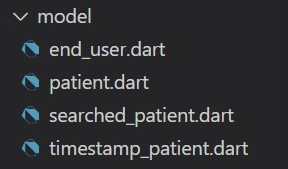
\includegraphics[scale = 1.0]{model}
\caption{The Model files}
\end{figure}
Il package Model contiene i vari oggetti utilizzati all'interno dell'applicazione che spesso si presentano con la presenza dei vari campi, del costruttore e di metodi di utilità generale per la classe. In particolare:
\begin{itemize}
\item end\_user: rappresenta l'utente finale dell'applicazione e permette di salvare le sue informazioni fondamentali ottenute da Firebase quali l'id, il codice fiscale, l'email e la tipologia di utente (cittadino o volontario);
\item patient: rappresenta il cittadino e contiene le informazioni invariabili (codice fiscale, nome e cognome) e una mappa di \texttt{TimestampPatient} organizzata per data con la funzione di storico per i dati precedenti a quelli attuali;
\item searched\_patient: rappresenta la classe utilizzata per gestire la ricerca dei cittadini da parte del volontario;
\item timestamp\_patient: contiene tutte le informazioni sanitarie e salvavita del cittadino relative ad una certa data e metodi di utilità per accedere ai dati.
\end{itemize}

\subsection{Screens}
Il package Screens contiene le schermate principali dell'applicazione. Ogni file corrisponde ad una schermata i cui widgets sono spesso contenuti nel package Widgets. In particolare:
\begin{itemize}
\item \texttt{emergency\_numbers}
\item \texttt{homepage}
\item \texttt{login}
\item \texttt{qr\_code\_scanner}
\item \texttt{volunteer}
\item \texttt{wrapper}
\end{itemize}

\subsection{Services}
Il package Services contiene le classi responsabili dei principali servizi utilizzati nelle varie schermate e nella logica dell'applicazione. In particolare:
\begin{itemize}
\item \texttt{auth\_service}
\item \texttt{database\_service}
\item \texttt{pdf\_handler}
\item \texttt{qr\_code\_handler}
\end{itemize}

\subsection{Widgets}

\section{Server-Side Application}
The server-side of the application is entirely hosted by \textbf{Google Firebase} that offers two main functionalities for the entire system:
\begin{itemize}
\item \textbf{Authentication}:
\item \textbf{Firestore Database}:
\end{itemize}
The best advantage is that Firebase and Flutter are both created by Google so it is very easy to implement the communication between them.

\subsection{Authentication}

\subsection{Firestore Database}
Diagramma ER.

\section{External Services and Libraries}
Durante la fase di sviluppo dell'applicazione mobile è stato fatto largo utilizzo dei packages forniti.


\chapter{Funzionalità}
\section{Panoramica dell'Applicazione}
L'applicazione è composta da una schermata principale e da un'insieme di pagine che forniscono diverse funzionalità. In particolare l'homepage è composta da 3 tabs il cui scopo è rispettivamente di:
\begin{enumerate}
\item mostrare il QR code contentente le informazioni salvavita del cittadino con la possiblità di aprirlo come immagine, salvarlo nel dispositivo o stamparlo;
\item mostrare i documenti originali generati dai dati sanitari e dalle informazioni salvavita del cittadino con la possibilità di aprirli, salvarli nel dispositivo o stamparli;
\item mostrare uno storico relativo agli ultimi eventi relativi all'argomento Covid del cittadino (come ad esempio i tamponi o le vaccinazioni effettuati) e un QR code che riassume tutti questi eventi.
\end{enumerate}
Oltre alla schermata principale sono presenti ulteriori funzionalità che permettono all'utente di:
\begin{itemize}
\item contattare il volontario e l'MMG responsabili dell'inserimento dei dati tramite email o numero telefonico;
\item avere una lista dei numeri utili di emergenza (quali forze dell'ordine, pronto soccorso, ...), con la possibilità di contattarli in caso di necessità;
\item scannerizzare un altro QR code attraverso uno scanner integrato all'applicazione con la possibilità di mostrare i dati salvavita di un altro cittadino. Questa funzionalità è pensata per essere utilizzata dai soccorritori in caso di necessità.
\end{itemize}
Oltre alle schermate appena descritte è presente un'intera parte dell'applicazione riservata al volontario con lo scopo di abilitare la ricerca di uno o più cittadini con la facoltà di stampare per essi i documenti generati dai loro dati.

\section{Descrizione delle Funzionalità}
Nelle sezioni successive verranno analizzate nel dettaglio le funzionalità introdotte nel paragrafo precedente cercando di mettere in luce gli scopi e i modi d'utilizzo pensati.

\subsection{Registrazione}
La registrazione degli accounts avviene in due modi fondamentali in base alla tipologie di utente:
\begin{itemize}
\item volontario: la creazione dell'account del volontario (e anche quello dell'MMG) avviene per mano dell'amministratore di sistema a seguito di una richiesta. In questo modo è possibile assicurare solamente alle persone corrette il privilegio di esercitare la propria professione e avere l'accesso ai dati sensibili dei cittadini;
\item cittadino: l'account del cittadino viene creato dal volontario a seguito dell'inserimento dei dati sanitari da parte dell'MMG. In questo modo il cittadino può avere accesso all'applicazione solo a seguito dell'inserimento dei suoi dati.
\end{itemize}
Le password degli accounts sono generate in maniera randomica e inoltrate agli utenti via mail. A seguito di ciò l'utente sarà libero di modificarla secondo le proprie preferenze.

\subsection{Login}
La schermata di Login permette agli utenti di accedere al sistema fornendo credenziali valide e fornite a seguito del processo di registrazione analizzato precedentemente. Gli utenti sono in grado di modificare la propria password cliccando su "Hai dimenticato la password?" che invierà all'utente una mail contenente un link per il reset della stessa. Sia il cittadino che il volontario condividono la stessa scheramta di Login. Il sistema controlla le credenziali e reindirizza l'utente alla schermata corretta.

\subsection{Schermata del Volontario}
Il volontario ha accesso ad una singola schermata nell'applicazione mobile in quanto la maggior parte delle sue facoltà sono correlate all'utilizzo dell'applicazione web. Il volontario tramite un'apposita barra di ricerca è in grado di ricercare attraverso nome o codice fiscale gli utenti di sua competenza e selezionarli. A seguito della selezione è in grado di eseguire la stampa dei documenti fondamentali (CIS, badge e braccialetto) del singolo o del gruppo di utenti selezionati.

\subsection{Homepage}
L'Homepage è la schermata principale dell'applicazione ha cui ha accesso il cittadino. Questa scheramta è suddivisa in 3 tabs principali che forniscono diverse funzionalità:
\begin{enumerate}
\item la prima tab mostra il QR code salvavita del cittadino contenente:
\begin{itemize}
\item Nome e cognome;
\item Data di nascita;
\item Gruppo sanguigno;
\item Primo contatto ICE;
\item Secondo contatto ICE;
\item Lista delle eventuali patologie;
\item Lista delle eventuali allergie;
\item Informazioni aggiuntive.
\end{itemize}
e permette all'utente di aprirlo come immagine, salvarlo nella galleria del dispositivo o stamparlo in formato .pdf;
\item la seconda tab mostra i documenti principali generati dai dati sanitari e salvavita inseriti dall'MMG e dal volontario incaricato:
\begin{itemize}
\item Profilo Sanitario Sintetico: contiene tutti i dati sanitari e salvavita relativi al cittadino;
\item Carta d'Identità Salvavita: mostra la CIS del cittadino contenente la foto, il QR code, i contatti ICE e le informazioni salvavita;
\item Badge: mostra la foto, il QR code e i contatti ICE;
\item Braccialetto: contiene i loghi delle società partner e il QR code.
\end{itemize}
\item la terza tab mostra gli eventi relativi alla storia Covid del cittadino, come ad esempio i tamponi effettuati o le vaccinazioni con la possibilità di aprire i documenti relativi inseriti dall'MMG o dal volontario. La schermata contiene anche un QR code riassuntivo dei vari eventi.
\end{enumerate}
Tramite l'Homepage il cittadino è in grado di accedere alle altre funzionalità dell'applicazione (accessibili anche dalla schermata di Login) o di disconnettersi.

\subsection{Numeri Utili}
La schermata dei Numeri Utili è accessibile sia dalla schermata di Login, sia dall'Homepage e presenta due funzionalità principali:
\begin{itemize}
\item permette al cittadino loggato di contattare l'MMG e il volontario incaricato della gestione dei suoi dati tramite email o numero telefonico;
\item provvede ad una lista di numeri di emergenza che possono essere contattati dall'utente in caso di necessità:
\begin{itemize}
\item carabinieri;
\item polizia di stato;
\item vigili del fuoco;
\item guarda di finanza;
\item emergenza sanitaria.
\end{itemize}
\end{itemize}

\subsection{Scanner QR Code}
La schermata dello Scanner è accessibile sia dalla schermata di Login, sia dall'Homepage. Questa funzionalità è stata pensata per essere utilizzata dai soccorritori che, senza dover necessariamente fare l'accesso all'applicazione, possono utilizzare lo scanner QR per avere accesso immediato alle informazioni salvavita dei cittadini in difficoltà. L'applicazione infatti, a seguito della scansione, mostra i dati del cittadino in forma leggibile ed organizzata.

\chapter{Interfaccia Utente e Casi d'Uso}
\section{UI Design}
Descrizione della UI e delle scelte prese in merito.

\section{Use Cases}


\subsection{Login}
\begin{table}[H]
\centering
\begin{tabular}{|p{3cm}|p{10.5cm}|}
\hline
Scenario & User's login \\
\hline
Entry condition & The user has downloaded the app or has accessed it using the web browser \newline
The user already has an account created by the volunteer \\
\hline
Flow of events & 
\begin{enumerate}
\item User fills in his email in the 'Email' field
\item User fills in his password in the 'Password' field
\item User clicks on the 'Login' button
\end{enumerate}\\
\hline
Exit condition & The application redirects the user to the Homepage of the application \\
\hline
Exceptions & 
\begin{itemize}
\item User did not insert valid personal information
\item User does not fill in all mandatory fields
\item The email address is already assigned to another account
\item The system is not able to complete the request due to an internal error
\end{itemize} \\
\hline
\end{tabular}
\end{table}

\subsection{Homepage}
\begin{table}[H]
\centering
\begin{tabular}{|p{3cm}|p{10.5cm}|}
\hline
Scenario & Life-Saving Information QR Code \\
\hline
Entry condition & The citizen is logged-in in the Homepage screen\\
\hline
Flow of events & 
\begin{enumerate}
\item User clicks on the "Apri" button
\item The application opens the full-screen image of the QR Code
\end{enumerate}\\
\hline
Exit condition & The application redirects the user to the Homepage of the application \\
\hline
Exceptions & 
\begin{itemize}
\item User did not insert valid personal information
\item User does not fill in all mandatory fields
\item The email address is already assigned to another account
\item The system is not able to complete the request due to an internal error
\end{itemize} \\
\hline
\end{tabular}
\end{table}

\subsection{Volunteer Screen}

\subsection{Useful Numbers}

\subsection{QR Code Scanner}

\section{User-Flow Diagram}


\chapter{Discussions and Conclusion}
Discussione sui risultati raggiunti e sulle possibili migliorie.

\chapter{Bibliografia}
Di seguito le fonti utilizzate per la stesura del documento e la realizzazione del progetto:
\begin{itemize}
\item \href{https://www.medicivolontaritaliani.org/}{Medici Volontari Italiani};
\item \href{https://www.comune.milano.it/aree-tematiche/servizi-sociali/raccolta-dati-personali-per-interventi-di-emergenza}{Comune di Milano};
\end{itemize}

\end{document}